\chapter{Lexicale Analyse}
\label{ch:lexicale_analyse}
\section{Lexicale tokens}
\begin{itemize}
	\item Herkennen van een reeks opeenvolgende karakters die een geheel vormen volgens de syntax van een programmeertaal, zoals o.a:
	\begin{itemize}
		\item sleutelwoorden: int, float, for, new, ...
		\item identifiers: foo, n14, variabelenaam
		\item getallen: -37, 0x16L, 10.4, ...
		\item operatoren: +, -, *, \&, \&\&, ...
		\item andere tokens: \{ \} " ; /*  */ / ( ) [ ]
	\end{itemize}
	\item Veronderstel volgende code:
	\begin{lstlisting}
float match0(char * s) {/* find a zero */ 
	if(!strncmp(s, "0.0", 3))
		return 0.;
}
	\end{lstlisting}
	, dan worden volgende tokens gegenereerd, waarbij dat sommige tokens een {\color{red}attribuut} hebben:
	\texttt{FLOAT ID({\color{red}match0}) LPAREN CHAR START ID({\color{red}s}) RPAREN LBRACE IF LPAREN BANG ID ({\color{red}strncmp}) LPAREN ID({\color{red}s}) COMMA STRING({\color{red}''0.0''}) COMMA NUM({\color{red}3}) RPAREN RPAREN  RETURN REAL({\color{red}0.0}) SEMI RBRACE EOF}
	\end{itemize}
\section{Eindige automaten}
	\begin{itemize}
	\item Er wordt met reguliere expressie gewerkt om te omschrijven welke karaktersequentie met een bepaald token overeenstemmen:
	
	\begin{table}[h]
		\centering
		\begin{tabular}{l l}
			$if$ & \{return IF;\} \\
			$[a-z][a-z0-9]*$ &\{return ID;\} \\
			$[0-9]+$ & \{return NUM;\} \\
			$([0-9]+"."[0-9]*)|([0-9]*"."[0-9]+)$ & \{return REAL;\} \\
		\end{tabular}
		\caption{Reguliere expressies voor een aantal tokens.}
		\label{table:reguliere_expressies_tokens}
	\end{table}

	\item Met behulp van de \underline{constructie van Thompson} kan een \textbf{niet-deterministische automaat (NFA)} opgebouwd worden uit een reguliere expressie. Op figuur \ref{fig:eindige_automaten} zijn de \underline{eindige automaten} te zien van de reguliere expressies uit tabel \ref{table:reguliere_expressies_tokens}.
	\begin{figure}
		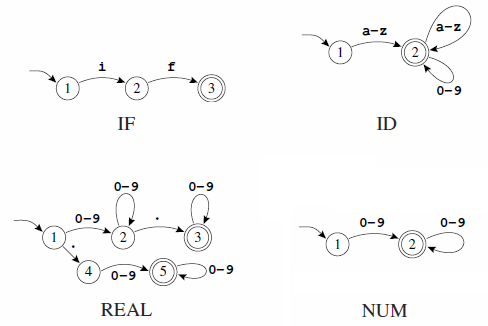
\includegraphics[width=\textwidth]{eindige_automaten}
		\caption{Eindige automaten voor lexicale tokens.}
		\label{fig:eindige_automaten}
	\end{figure}

	\item Deze individuele automaten kunnen samengevoegd worden tot een gecombineerde automaat, te zien op figuur \ref{fig:deterministische_eindige_automaat}
		\begin{figure}
		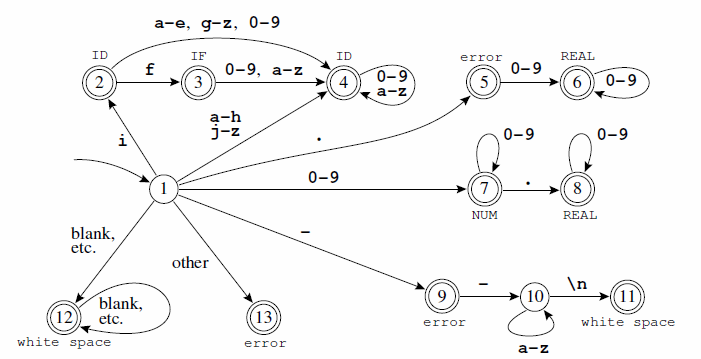
\includegraphics[width=\textwidth]{deterministische_eindige_automaat}
		\caption{Combinatie van eindige automaten.}
		\label{fig:deterministische_eindige_automaat}
	\end{figure}

	In dit geval is de gecombineerde automaat al een \textbf{deterministische eindige automaat (DFA)} aangezien elke mogelijke staat slechts één transitie heeft voor elke input. Het doel van lexicale analyse is om een DFA op te stellen zodat de tokens op een efficiënte manier kunnen bepaald worden. Een DFA wordt doorgaans geïmplementeerd als een transitietabel:
	\begin{lstlisting}
int edges[][256] = { /* ... 0 1 2 ... - ... e f g h i j ... */ 
/* state 0 */      {    ... 0 0 0 ... 0 ... 0 0 0 0 0 0 ...},
/* state 1 */      {    ... 7 7 7 ... 9 ... 4 4 4 4 2 4 ...},
/* state 2 */      {    ... 4 4 4 ... 0 ... 4 3 4 4 4 4 ...},
/* state 3 */      {    ... 4 4 4 ... 0 ... 4 4 4 4 4 4 ...},
/* state 4 */      {    ... 4 4 4 ... 0 ... 4 4 4 4 4 4 ...},
/* state 5 */      {    ... 6 6 6 ... 0 ... 0 0 0 0 0 0 ...},
/* state 6 */      {    ... 6 6 6 ... 0 ... 0 0 0 0 0 0 ...},
/* state 7 */      {    ... 7 7 7 ... 0 ... 0 0 0 0 0 0 ...},
/* state 8 */      {    ... 8 8 8 ... 0 ... 0 0 0 0 0 0 ...},
/* ... */
};
	\end{lstlisting}
\end{itemize}

\section{Opbouw deterministische eindige automaat}
\begin{itemize}
	\item We starten met een reguliere expressie, die een bepaald token voorstelt:
	
	$$\texttt{(aaa)*|(aa)*}$$
	
	\item Zoals vermeld zal de constructie van Thompson een niet-deterministische automaat aanmaken van een bepaalde reguliere expressie. Er bestaat de kans dat deze automaat deterministisch is, maar dat is niet altijd zo. In het geval van bovenstaande reguliere expressie ziet de automaat er uit zoals op figuur \ref{fig:niet_deterministische_automaat} of figuur \ref{fig:niet_deterministische_automaat_e}.
	\begin{figure}[h]
		\centering
		\begin{minipage}{0.7\textwidth}
			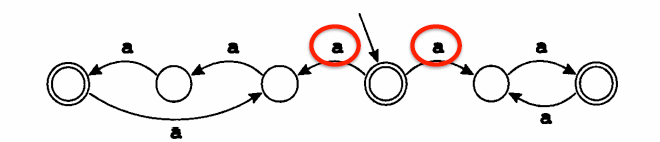
\includegraphics[width=\textwidth]{niet_deterministische_automaat}
			\caption{Een niet-deterministische eindige automaat.}
			\label{fig:niet_deterministische_automaat}
		\end{minipage}
		\begin{minipage}{0.7\textwidth}
			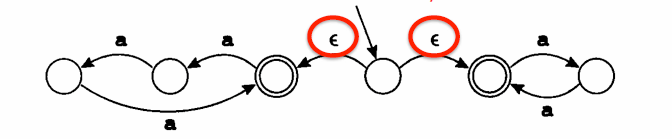
\includegraphics[width=\textwidth]{niet_deterministische_automaat_e}
			\caption{Een niet-deterministische eindige automaat waarbij de eerste transitie kan gebeuren zonder een symbool te verwerken.}
			\label{fig:niet_deterministische_automaat_e}
		\end{minipage}
	\end{figure}

	Welke richting moeten we nu uit bij \texttt{aaaaaaaa} voor de eerste \texttt{a}? Bij een niet-deterministische automaat moeten we gokken welke de juiste zal zijn.
	
	\item Gelukkig kan ook een DFA opgebouwd worden uit een NFA via de \underline{deelverzamelingconstructie}. Op die manier kan een DFA opgebouwd worden door (i) enkel de reguliere expressies handmatig te definiëren, (ii) algoritmisch deze reguliere expressies om te vormen tot een NFA, en (iii) algoritmisch deze NFA om te vormen tot een DFA. 
	
	\item Veronderstel de reguliere expressies en de daarbijhorende NFA in figuur \ref{fig:nfa_to_dfa}.
	\begin{figure}[h]
		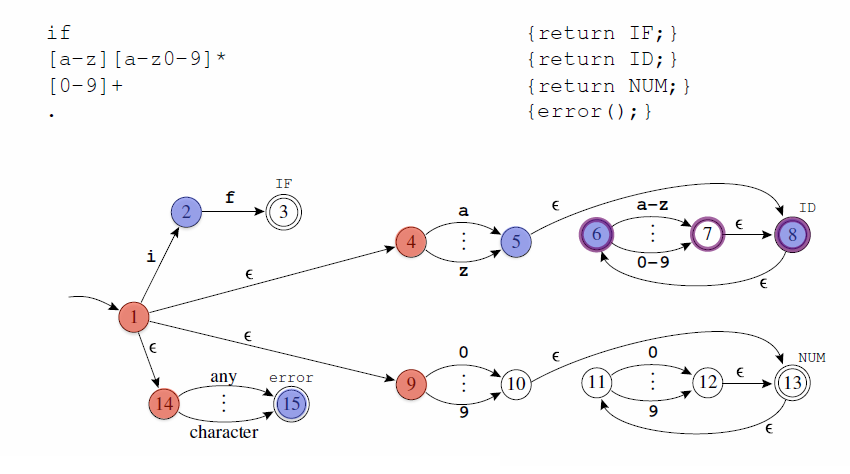
\includegraphics[width=\textwidth]{nfa_to_dfa}
		\caption{Een aantal reguliere expressies en de daarbijhorende NFA.}
		\label{fig:nfa_to_dfa}
	\end{figure}

	Stel dat we nu de string \textit{in} moeten checken:
	\begin{enumerate}
		\item Zonder teken op te eten kunnen we in 1 komen en in zijn $\epsilon$-closure: {\color{red}\{1, 4, 9, 14\}}.
		\item Vanuit {\color{red}\{1, 4, 9, 14\}} kunnen we voor \textit{i} naar {\color{blue}\{2, 5, 6, 8, 15\}}.
		\item Vanuit {\color{blue}\{2, 5, 6, 8, 15\}} kunnen we voor \textit{n} naar {\color{purple}\{6, 7, 8\}}.
		\item Daarvan is 8 een aanvaardingstoestand voor \texttt{ID}.
	\end{enumerate}
	Op die manier bekomen we de DFA uit figuur \ref{fig:nfa_geconverteerd_dfa}.
	\begin{figure}[h]
		\centering
		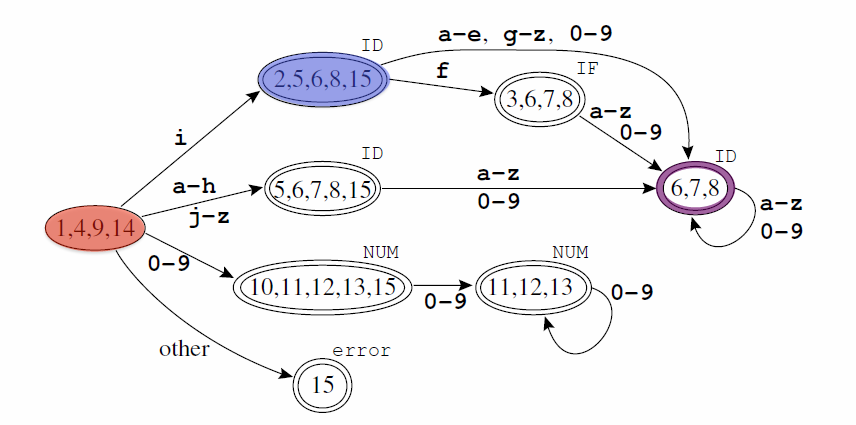
\includegraphics[width=0.8\textwidth]{nfa_geconverteerd_dfa}
		\caption{De NFA uit figuur \ref{fig:nfa_to_dfa} geconverteerd naar een DFA.}
		\label{fig:nfa_geconverteerd_dfa}
	\end{figure}
\end{itemize}
\subsection{Conversie NFA naar DFA}
\begin{itemize}
	\item Drie functies:
	\begin{enumerate}
		\item \textbf{edge(s, c)} = alle NFA staten bereikbaar uit toestand $s$ over pijlen met transitiesymbool $c$.
		\item \textbf{closure(S)} = de kleinste verzameling $T$ voor een subset $S$ waarvoor geldt:
		$$
		T = S \cup \bigg(\bigcup_{s \in T} \hbox{\textbf{edge}}(s, \epsilon)\bigg)
		$$
		
		\QA{Waarom moet dit de kleinste verzameling zijn?}
		{De volledige verzameling van toestanden voldoet ook aan deze vergelijking, en dat is een triviaal geval.}
		
		Via iteratie kan $T$ berekent worden:
			\begin{lstlisting}[escapeinside={(*}{*)}]
(*$T \leftarrow S$*)
(*\textbf{repeat}*)
  (*$T' \leftarrow T$*)
  (*$T \leftarrow T' \cup (\bigcup_{s \in T'} \hbox{\textbf{edge}}(s, \epsilon))$*)
(*\textbf{until} T = T'*)
			\end{lstlisting}
			
		\begin{itemize}
			\item Dit is een voorbeeld van een \underline{fixpoint algoritme}. Dit wil zeggen dat uiteindelijk $f(x) = x$ geldig is. In het voorbeeld van de functie \textbf{closure(S)}, hier genoteerd als \textbf{F(x)}, is dit zeker waar:
			\begin{equation*}
				\begin{split}
					F(\epsilon) & = S \\
					F(S) & = ... \\
					F(F(S)) & = ...\\
					...\\
					F(F(F(...))) & = T \\
					F(T) & = T
				\end{split}
			\end{equation*}
			\item Aangezien dat uiteindelijk $F(T) = T$ en dat er maar een eindig aantal staten zijn zal het algoritme zeker stoppen.
		\end{itemize}
	
		\item Veronderstel dat we ons bevinden in een set $d = \{s_i, s_k, s_l\}$ van NFA staten $s_i, s_k$ en $s_l$. Startend vanuit $d$ en het symbool $c$, bekomen we een nieuwe set van NFA staten:
		$$\hbox{\textbf{DFAedge(D, c)}} = \hbox{\textbf{closure}}\bigg(\bigcup_{s \in D} \hbox{\textbf{edge}}(s, c)\bigg)$$
		
		Via deze functie, de startstaat $s_1$ en input string $c_1, ..., c_k$ kan de NFA simulatie als volgt geschreven worden:
			\begin{lstlisting}[escapeinside={(*}{*)}]
(*$d \leftarrow \hbox{\textbf{closure}}(\{s_1\})$*)
(*$\hbox{\textbf{for}} i \leftarrow 1\;\hbox{\textbf{to}}\;k$*)
  (*$d \leftarrow \hbox{\textbf{DFAedge}}(d, c_i)$*)
			\end{lstlisting}
	
		
	\end{enumerate}
	\item De combinatie van deze drie functies leiden tot het algoritme om een NFA om te zetten naar een DFA:
	\begin{lstlisting}[escapeinside={(*}{*)}]
(*$\hbox{states[0]} \leftarrow \{\};$*)
(*$\hbox{states[1]} \leftarrow \hbox{\textbf{closure}}(\{s_1\});$*)
(*$p \leftarrow 1;\qquad j \leftarrow 0;$*)
(*$\hbox{\textbf{while}} j \leq p$*)
  (*$\hbox{\textbf{foreach}}\;c \in \Sigma$*)
  (*$e \leftarrow \hbox{\textbf{DFAedge}}(\hbox{states[j]}, c)$*)
  (*$\hbox{\textbf{if}}\;e == \hbox{states[i]}\;\hbox{for some}\; i\leq p$*)
    (*$\hbox{\textbf{then}}\;\hbox{trans[j, c]} \leftarrow i$*)
    (*$\hbox{\textbf{else}}\;p \leftarrow p + 1$*)
      (*$\hbox{states[p]} \leftarrow e$*)
      (*$\hbox{states[j,c]} \leftarrow p$*)
(*$j \leftarrow j +1$*)
	\end{lstlisting}
	De gegenereerde DFA is suboptimaal: vanuit sommige toestanden worden identiek dezelfde strings aanvaard. 
\end{itemize}



